
% Лабораторная работа по криптографии № 1
% Михедов Константин Константинович

% Тип документа: статья, на бумаге А4
\documentclass[a4paper]{article}

% Подключение сторонних tex файлов 
\usepackage{import}


% Основные данные - ВУЗ, факультет, город...
\import{./../../stuff/tex}{config.tex}
% Небольшой набор инструментов
\import{./../../stuff/tex}{tools.tex}

% Подключение необходимых зависимостей
\import{./../../stuff/tex/settings}{packages.tex}
% Настройка подключенных пакетов
\import{./../../stuff/tex/settings}{preferences.tex}


% Шаблон титульной страницы 
\import{./../../stuff/tex/templates}{title.tex}
% Упрощенный блок "выполнил"
\import{./../../stuff/tex/templates}{sign2.tex}
% Макрос для содержания
\import{./../../stuff/tex/templates}{toc.tex}

% Определяем название документа
\title{
  ОТЧЕТ \\
  О ПРАКТИЧЕСКОЙ РАБОТЕ №1 \\
  по дисциплине <<Основы криптографии и стеганографии>> \\
  ПОДСТАНОВОЧНЫЕ ШИФРЫ  
}
% Указываем преподавателя
\renewcommand{\teachername}{
    Заведующий кафедрой информационной безопасности киберфизических систем \\
    канд. техн. наук, доцент \\
    \entryline{3.5cm} О.О. Евсютин
}


% Путь до внешних изображений
\graphicspath{ {./figures/}}
% Нумеруем все формулы
\mathtoolsset{showonlyrefs=false}


% Основной текст работы
\begin{document}
  \templatedtitlepage
  
  \toc

  \section{Здание на практическую работу}

  Целью данной практической работы является программная реализация и последующий 
  криптоанализ некоторых подстановочных шифров.

  В рамках работы необходимо выполнить следующие шаги:

  \begin{enumerate}
    \setlength{\itemindent}{1cm}
    \item {
        Программно реализовать следующие подстановочные шифры 

        \begin{itemize}
            \setlength{\itemindent}{1cm}
            \item Шифр простой замены
            \item Аффинный шифр 
            \item Рекуррентный Аффинный шифр
        \end{itemize}
    }
    \item {
        Изучить и описать методы криптографического анализа данных шифров 
    }
    \item {
        Провести криптоанализ данных шифров
    }
    \item {
        Подготовить отчет о проделанной работе
    }
  \end{enumerate}
  \newpage

  \section{Краткая теоретическая часть}

  \subsection{Описание шифров}

  \subsubsection{Шифр простой замены}

  Является одним из наиболее простых в реализации и понимании шифров. Допустим,
  имеется некоторое сообщение $X$ длиной $n$ символов: $X = (x_1, x_2, \dots, x_n)$,
  где $x_i$ - $i$-ый символ данного сообщения, причем каждый символ этого сообщения принадлежит 
  алфавиту $A$ мощности $m$.

  Для получения шифртекста необходимо задать ключ - перестановку $k$ вида (\ref{eq:k_sp}).
  \begin{equation}
    k = \begin{pmatrix}
        a_1 & a_2 & \dots & a_m \\
        a_{l_1} & a_{l_2} & \dots & a_{l_m}
    \end{pmatrix}
    \label{eq:k_sp}
  \end{equation}

  Тогда определяются операции зашифрования (\ref{eq:en_sp}) и расшифрования (\ref{eq:de_sp}):
  \begin{equation}
    E_k(X) = E_k(x_1, x_2, \dots, x_n) = (k(x_1), k(x_2), \dots, k(x_n))
    \label{eq:en_sp}
  \end{equation}
  \begin{equation}
    D_k(Y) = D_k(y_1, y_2, \dots, y_n) = (k^{-1}(y_1), k^{-1}(y_2), \dots, k^{-1}(y_n))
    \label{eq:de_sp}
  \end{equation}

  В формуле (\ref{eq:de_sp}) $Y$ - шифртекст исходного сообщения $X$, полученный в результате
  зашифрования (формально $Y = E_k(X)$).

  \subsubsection{Аффинный шифр}

  Снова введем алфавит $A$ мощности $m$, исходное сообщения $X = (x_1, x_2, \dots, x_n)$ длины $n$
  и шифртекст данного сообщения $Y = (y_1, y_2, \dots, y_n)$ той же длины.

  Для определения операций шифрования и расшифрования необходимо ввести ключ - 
  пару чисел $k$ вида $(\alpha, \beta)$ такую, что НОД($\alpha$, $m$) = 1.

  Тогда операции шифрования (\ref{eq:en_aff_s}) и расшифрования (\ref{eq:de_aff_s}) отдельного символа описываются следующим образом:
  \begin{equation}
    E_k(x_i) = (\alpha x_i + \beta) \mod{m} = y_i
    \label{eq:en_aff_s}
  \end{equation}
  \begin{equation}
    D_k(y_i) = ((y_i - \beta) \times (\alpha^{-1} \mod{m}))\mod{m} = x_i
    \label{eq:de_aff_s}
  \end{equation}

  Из операций для отдельного символа можно вывести описания зашифрования (\ref{eq:en_aff}) и расшифрования (\ref{eq:de_aff}) целого текста:
  \begin{equation}
    E_k(X) = E_k(x_1, x_2, \dots, x_n) = (E_k(x_1), E_k(x_2), \dots, E_k(x_n))
    \label{eq:en_aff}
  \end{equation}
  \begin{equation}
    D_k(Y) = D_k(y_1, y_2, \dots, y_n) = (D_k(y_1), D_k(y_2), \dots, D_k(y_n))
    \label{eq:de_aff}
  \end{equation}

  \subsubsection{Рекуррентный Аффинный шифр}

  Данный шифр очень похож на обычный Аффинный шифр, разница лишь в том, что ключа $k$ - 
  свой для каждого символа.

  Для данного шифра опять таки потребуется алфавит $A$ мощности $m$, исходное сообщение 
  $X = (x_1, x_2, \dots, x_n)$ длины $n$. Также определим вид шифртекста: 
  $Y = (y_1, y_2, \dots, y_n)$.

  Далее введем два первичных ключа: $k_1 = (\alpha_1, \beta_1)$ и $k_2 = (\alpha_2, \beta_2)$, причем
  эти ключи должны быть такими, что НОД$(\alpha_1, m) = $ НОД$(\alpha_2, m) = 1$.

  Теперь задаем рекуррентную формулу для получения ключа для $i$-ого символа (\ref{eq:raff_k}):
  \begin{equation}
    k_i = (\alpha_{i - 1} \times \alpha_{i - 2}, \beta_{i - 1} + \beta_{i - 2}) \:\:\: \forall \:\: i \geq 3 \land i \in \mathbb{N}
    \label{eq:raff_k}
  \end{equation}

  Переопределяем операции зашифрования (\ref{eq:en_raff}) и расшифрования (\ref{eq:de_raff}) одного символа:
  \begin{equation}
    E_k(x_i) = (\alpha_ix_i + \beta_i)\mod{m} = y_i
    \label{eq:en_raff}
  \end{equation}
  \begin{equation}
    D_k(y_i) = ((y_i - \beta_i) \times (\alpha_i^{-1}\mod{m}))\mod{m} = x_i
    \label{eq:de_raff}
  \end{equation}

  Зашифрование и расшифрование в общем виде совпадает с Аффинным шифром.

  \subsection{Методы криптографического анализа}

  \subsubsection{Метод грубой силы}

  Наиболее примитивным методом является метод грубой силы. Его суть заключается в полном переборе всех
  возможных ключей до тех пор, пока не будет найден тот, с помощью которого производилось зашифрование.

  Найти необходимую перестановку для шифра простой замены может быть достаточно сложно, по причине
  огромного количества этих самых перестановок. Для английского алфавита, состоящего только из маленьких
  букв, в худшем случае потребуется перебрать $26!$ различных вариантов (приблизительно $4 \times 10^{26}$).
  Соответственно, для достаточно большого по мощности алфавита данный способ практически бесполезен.

  Для Аффинного шифра потребуется перебирать уже не перестановки алфавита, а числа $\alpha$ и $\beta$,
  с помощью который производилось шифрование. Так как зашифрование каждого символа происходит
  по модулю мощности алфавита, не имеет смылса рассматривать числа $\beta$ большие, чем эта
  самая мощность алфавита. Перебор также упрощает факт того, что НОД$(\alpha, m) = 1$, отсеивается
  достаточно большое количество различных чисел для проверки. Поэтому метод грубой силы при 
  взломе Аффинного шифра может иметь достаточно высокую эфективность.

  Рекуррентный Аффинный шифр всего лишь добавляет к перебору еще одну пару вида $(\alpha, \beta)$,
  поэтому метод грубой силы для него релевантен так же, как и для обычного Аффинного шифра.

  \subsubsection{Частотный анализ}

  Шифр просто замены и Аффинный шифр в своей реализации получают строгую биекцию вида символ-символ
  при помощи которой выполняется замена. Это соответствие не меняется по ходу зашифрования, поэтому 
  каждая определенная буква станет дургой, также строго определенной буквой. При таком подходе
  сохраняются общие характеристики исходного текста - в особенности, частота использования
  какого-либо символа (символ по факту другой, но используется с той же частотой, что и исходный).

  Для достаточно больших шифртекстов можно проследить закономерности, выделить, с какой частотой появляются
  те или иные символы и сопоставить эти вероятности с вероятностями использования символов в реальных текстах.
  На основе этого сравнения можно с определенной долей вероятности восстановить исходный текст.

  У рекуррентного Аффинного шифра нет четкой биективной подстановки, с помощью которой можно 
  сделать однозначный вывод какой символ на какой заменен, поэтому он устойчив к частотному анализу.

  \subsubsection{Атака на основе открытого текста}

  Если к злоумышленнику в руки попадает откртый текст или его часть, то в некоторых случаях
  можно будет при его помощи найти ключ.

  Так, если количество различных символов в полученном куске открытого текста близко к количеству
  символов в алфавите, и можно устноавить, какая часть шифртекста соответствует этому куску, то 
  можно будет без труда определить ключ и с его помощью произвести дорасшифровку.

  Аффинный шифр при таком же раскладе потребует найти решение системы нескольких уравнений.
  Это решение будет являться ключом, с помощью которого можно будет произвести дорасшифровку.

  У рекуррентного Аффинного шифра всего лишь потребуется решить на несколько уравнений больше, чтобы
  найти два ключа для двух подрядидущих символов. На их основе можно будет расшифровать ту 
  часть текста, которая идет после той, на основе которой были вычисленны ключи.

  \newpage

  \section{Примеры ручного шифрования}

  В качестве алфавита будет использоваться английкий, состоящий только из маленьких букв.
  Его мощность составляет 26 символов.

  Также установим, что нумерация букв в алфавите начинается с 0.

  \subsection{Шифр простой замены}

  Для первого примера зашифруем строку "hello world" с использованием следующего ключа:
  \begin{equation}
    k = \begin{pmatrix}
        a \:\: b \:\: c \:\: d \:\: e \:\: f \:\: g \:\: h \:\: i \:\: j \:\: k \:\: l \:\: m \:\: n \:\: o \:\: p \:\: q \:\: r \:\: s \:\: t \:\: u \:\: v \:\: w \:\: x \:\: y \:\: z \\
        b \:\: c \:\: d \:\: e \:\: f \:\: g \:\: h \:\: i \:\: j \:\: k \:\: l \:\: m \:\: n \:\: o \:\: p \:\: q \:\: r \:\: s \:\: t \:\: u \:\: v \:\: w \:\: x \:\: y \:\: z \:\: a
        %b & c & d & e & f & g & h & i & j & k & l & m & n & o & p & q & r & s & t & u & v & w & x & y & z & a
    \end{pmatrix}
    \label{eq:sp_k1}
  \end{equation}

  Из данной перестановки (\ref{eq:sp_k1}) видно, что каждая буква h будет заменена на i,
  e на f, l на m, o на p, w на x, r на s, d на e,
  и в результате зашифрования мы получим строку с шифртекстом - "ifmmp xpsme".

  Расшифровка заключается в обратной замене.

  \subsection{Аффинный шифр}

  Мощность алфавита 26, значит в качестве ключа нужно выбирать такую пару $(\alpha, \beta)$,
  что НОД$(\alpha, 26) = 1$. Прекрасно подойдет, например, ключ $(7, 4)$.

  Для зашифрования возьмем слово "master". Каждой букве в соответствие поставим ее
  порядковый номер: m - 12, a - 0, s - 18, t - 19, e - 4, r - 17. Для каждой буквы 
  поочередно выполним операцию зашифрования:
  \begin{equation}
    m: (12 * 7 + 4) \mod{26} = 10 (k)  
  \end{equation}
  \begin{equation}
    a: (0 * 7 + 4) \mod{26} = 4 (e)
  \end{equation}
  \begin{equation}
    s: (18 * 7 + 4) \mod{26} = 0 (a)
  \end{equation}
  \begin{equation}
    t: (19 * 7 + 4) \mod{26} = 7 (h)
  \end{equation}
  \begin{equation}
    e: (4 * 7 + 4) \mod{26} = 6 (g)
  \end{equation}
  \begin{equation}
    r: (17 * 7 + 4) \mod{26} = 19 (t)
  \end{equation}

  Результатом зашифрования является строка "keahgt".

  Для расшифровки потребуется найти $\alpha^{-1}\mod{26} = 7^{-1}\mod{26} = 15$.
  В качетсве проверки: $7 * 15 = 105$, а $105 \mod{26} = 1$. Тогда выполним расшифровку:
  \begin{equation}
    k: ((10 - 4) * 15) \mod{26} = 12 (m)
  \end{equation}
  \begin{equation}
    e: ((4 - 4) * 15) \mod{26} = 0 (a)
  \end{equation}
  \begin{equation}
    a: ((0 - 4) * 15) \mod{26} = 18 (s)
  \end{equation}
  \begin{equation}
    h: ((7 - 4) * 15) \mod{26} = 19 (t)
  \end{equation}
  \begin{equation}
    g: ((6 - 4) * 15) \mod{26} = 4 (e)
  \end{equation}
  \begin{equation}
    t: ((19 - 4) * 15) \mod{26} = 17 (r)
  \end{equation}

  Дешифровка дала правильный результат.

  \subsection{Рекуррентный Аффинный шифр}

  На этот раз необходимо два ключа, для примера возьмем ключи $(1, 3)$ и $(3, 1)$.
  (Важно, что НОД(3, 26) = НОД(1, 26) = 1)

  Зашифровывать будем слово "cringe". Для начала также необходимо найти порядковые номера
  букв: c - 2, r - 17, i - 8, n - 13, g - 6, e - 4. Далее необходимо вычислить ключи:
  \begin{equation}
    k_1 = (1, 3), \:\:\: k_2 = (3, 1)
  \end{equation}
  \begin{equation}
    k_3 = (1 \times 3, 3 + 1) = (3, 4)
  \end{equation}
  \begin{equation}
    k_4 = (3 \times 3, 4 + 1) = (9, 5)
  \end{equation}
  \begin{equation}
    k_5 = (9 \times 3, 5 + 4) = (27, 9)
  \end{equation}
  \begin{equation}
    k_6 = (27 \times 9, 9 + 5) = (243, 14)
  \end{equation}

  Далее произведем зашифрование при помощи полученных ключей:
  \begin{equation}
    c: (2 * 1 + 3) \mod{26} = 5 (f)
  \end{equation}
  \begin{equation}
    r: (17 * 3 + 1) \mod{26} = 0 (a)
  \end{equation}
  \begin{equation}
    i: (8 * 3 + 4) \mod{26} = 2 (c)
  \end{equation}
  \begin{equation}
    n: (13 * 9 + 5) \mod{26} = 18 (s)
  \end{equation}
  \begin{equation}
    g: (6 * 27 + 9) \mod{26} = 15 (p)
  \end{equation}
  \begin{equation}
    e: (4 * 243 + 14) \mod{26} = 24 (y)
  \end{equation}

  В результате зашифрования получается последовательность "facspy".

  \newpage

  \section{Программная реализация}

  Наиболее интересной частью программной реализации является нахождения обратного
  по модулю числа. Для этой опреации используется расширенный алгоритм Евклида,
  он же используется и пр подсчете НОД.

  \subsection{Шифр простой замены}

  \begin{figure}[H]  
    \centering
    \caption{Устанавливаем ключ}
    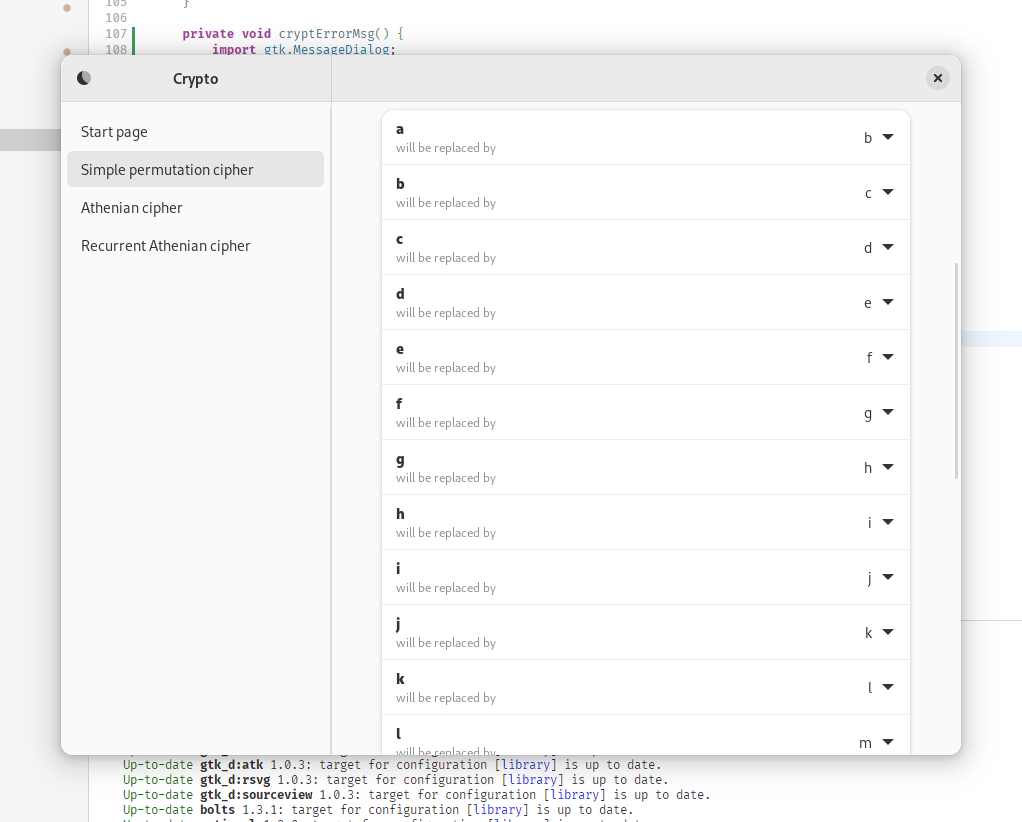
\includegraphics[width=0.8\textwidth]{01_0001}
    \label{img:0001}
  \end{figure}

  \begin{figure}[H]  
    \centering
    \caption{Вводим исходный текст}
    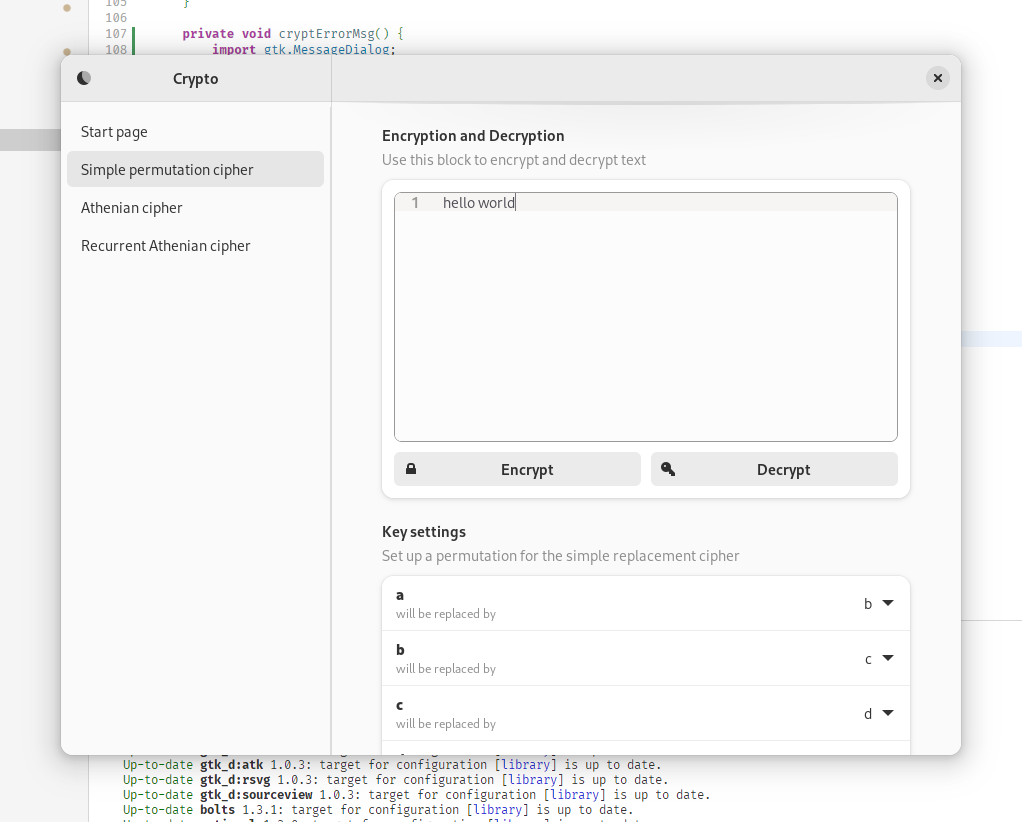
\includegraphics[width=0.8\textwidth]{01_0003}
    \label{img:0003}
  \end{figure}

  \begin{figure}[H]  
    \centering
    \caption{Зашифрование}
    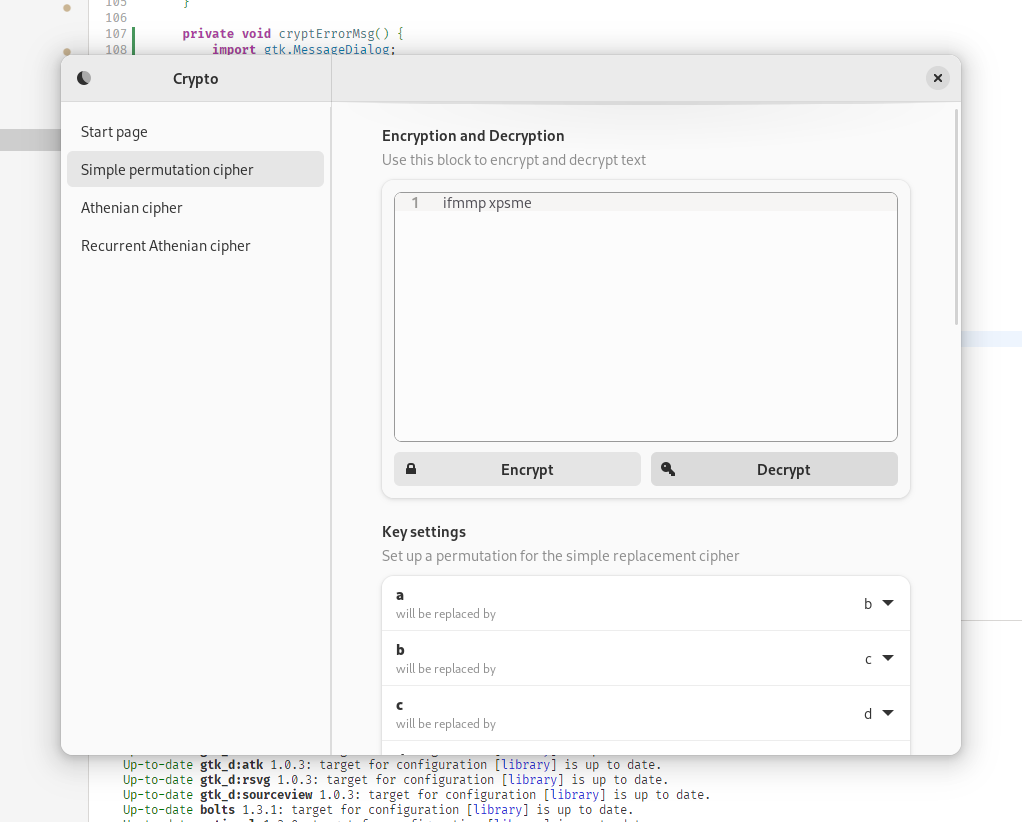
\includegraphics[width=0.8\textwidth]{01_0004}
    \label{img:0004}
  \end{figure}

  \begin{figure}[H]  
    \centering
    \caption{Расшифрование}
    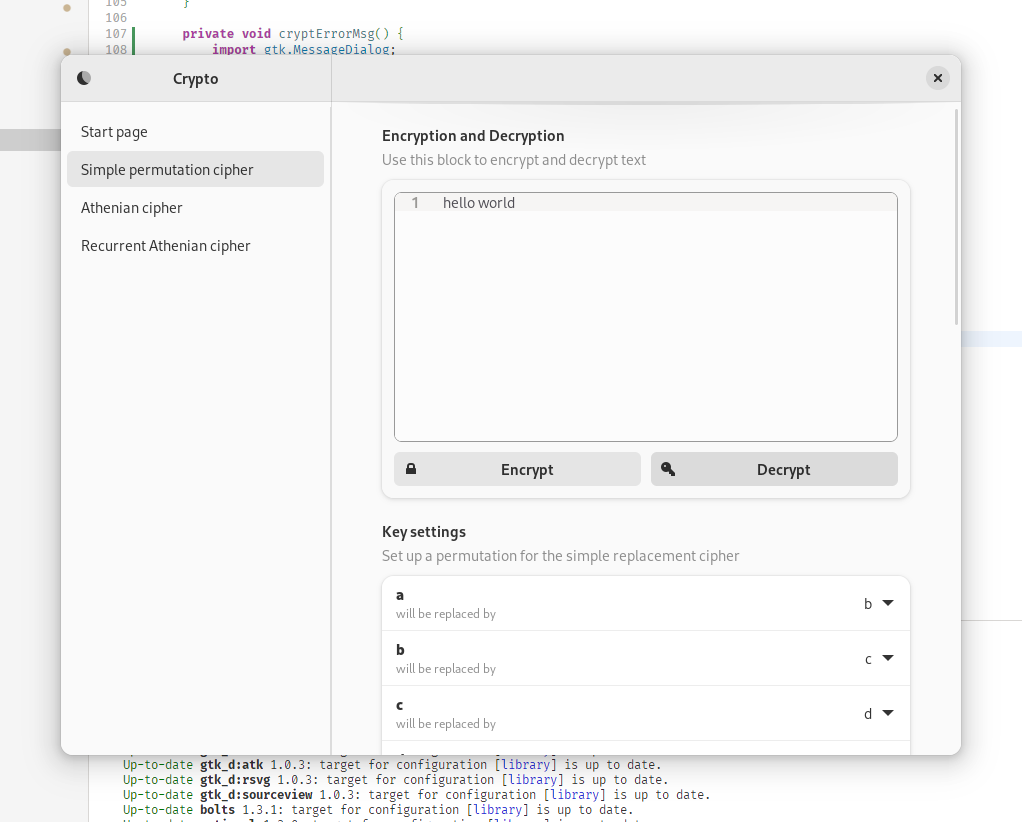
\includegraphics[width=0.8\textwidth]{01_0005}
    \label{img:0005}
  \end{figure}

  \subsection{Аффинный шифр}

  \begin{figure}[H]  
    \centering
    \caption{Устанавливаем ключ}
    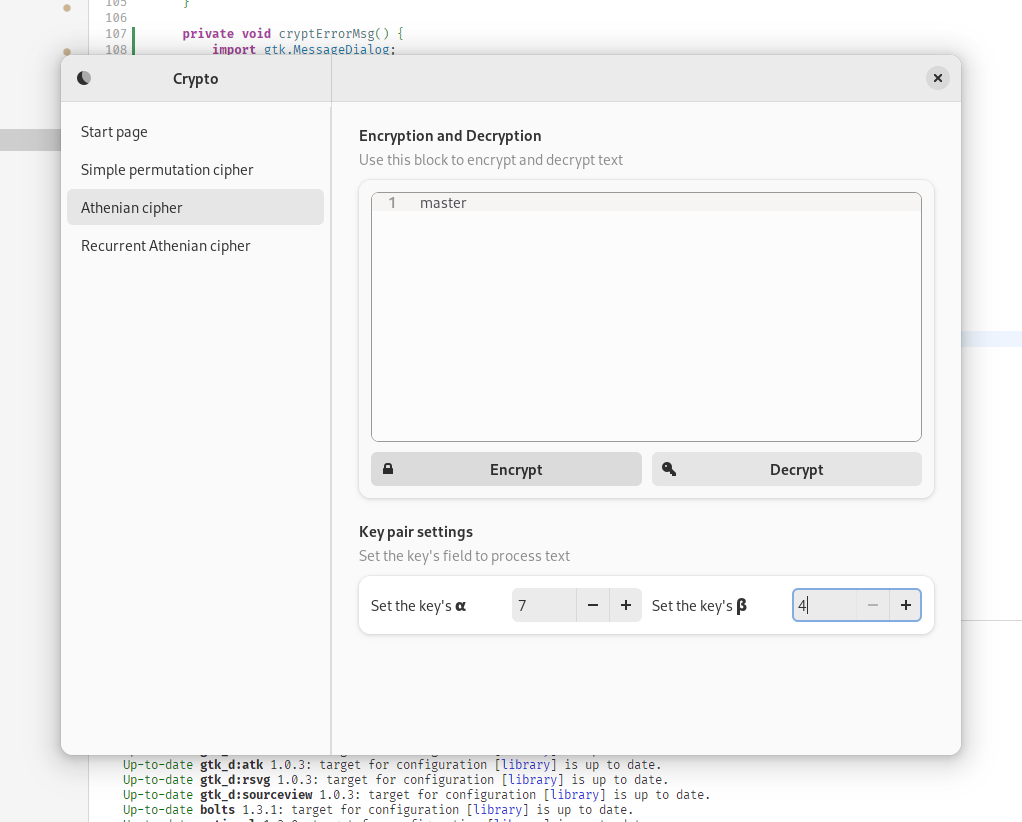
\includegraphics[width=0.8\textwidth]{01_0006}
    \label{img:0006}
  \end{figure}

  \begin{figure}[H]  
    \centering
    \caption{Зашифрование}
    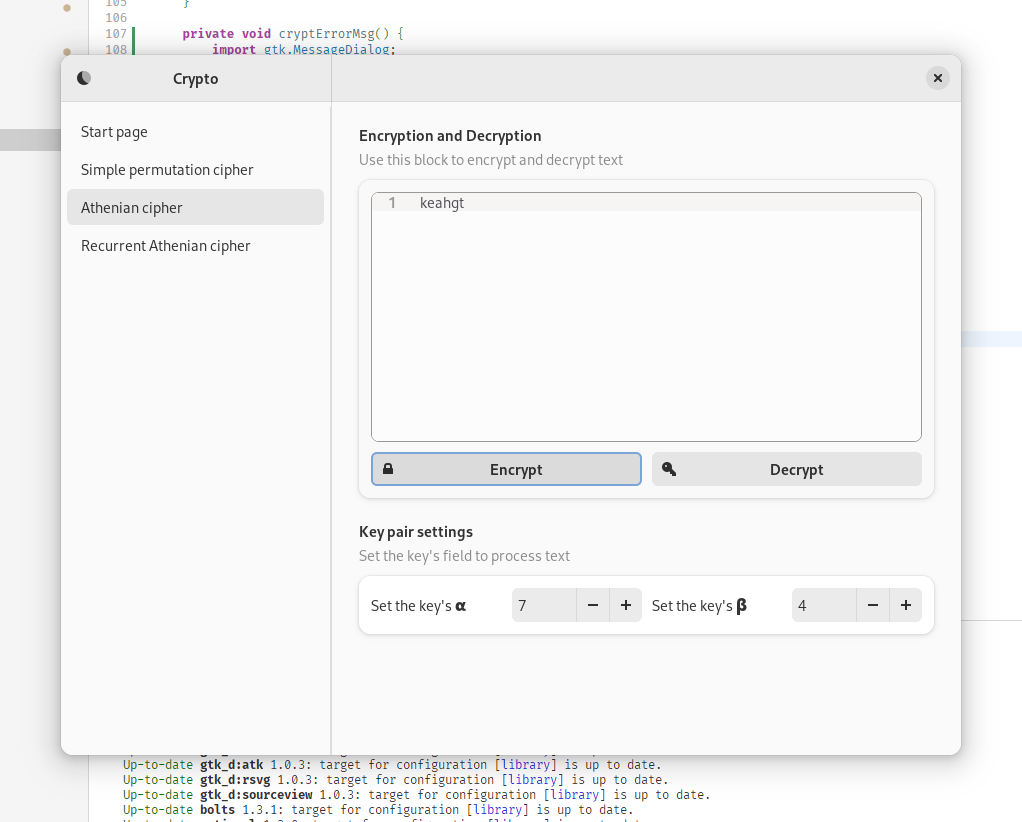
\includegraphics[width=0.8\textwidth]{01_0007}
    \label{img:0007}
  \end{figure}

  \begin{figure}[H]  
    \centering
    \caption{Расшифрование}
    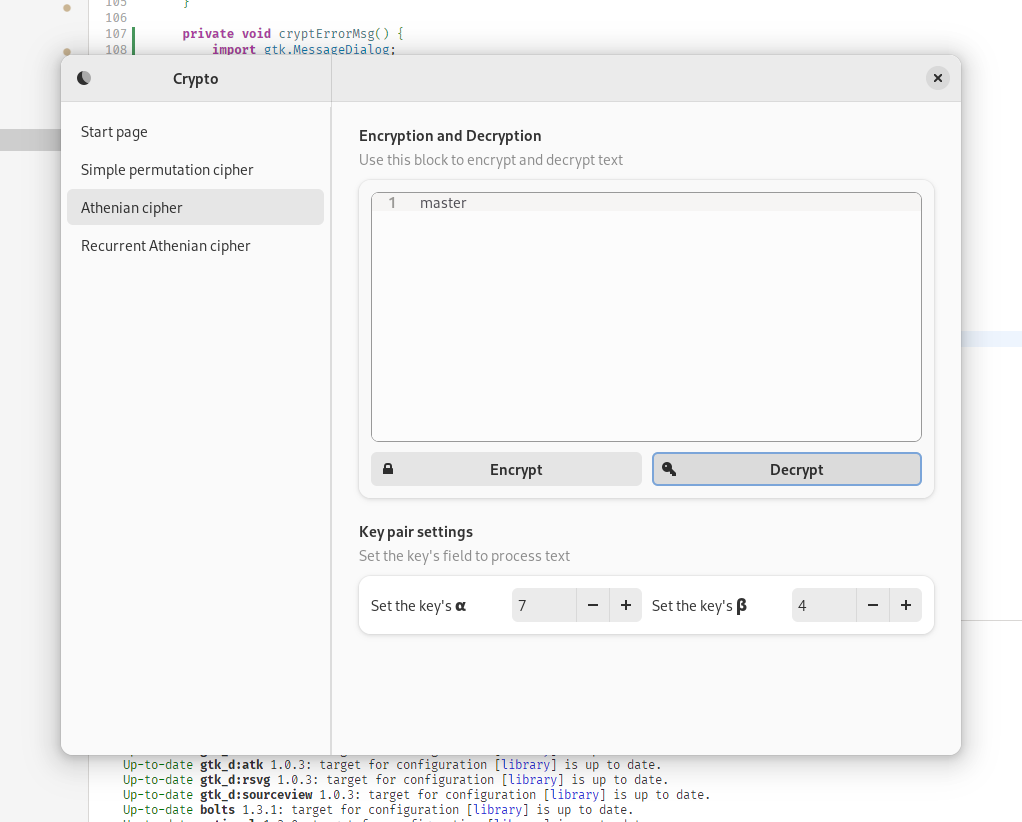
\includegraphics[width=0.8\textwidth]{01_0008}
    \label{img:0008}
  \end{figure}

  \subsection{Рекуррентный Аффинный шифр}

  \begin{figure}[H]  
    \centering
    \caption{Устанавливаем ключ}
    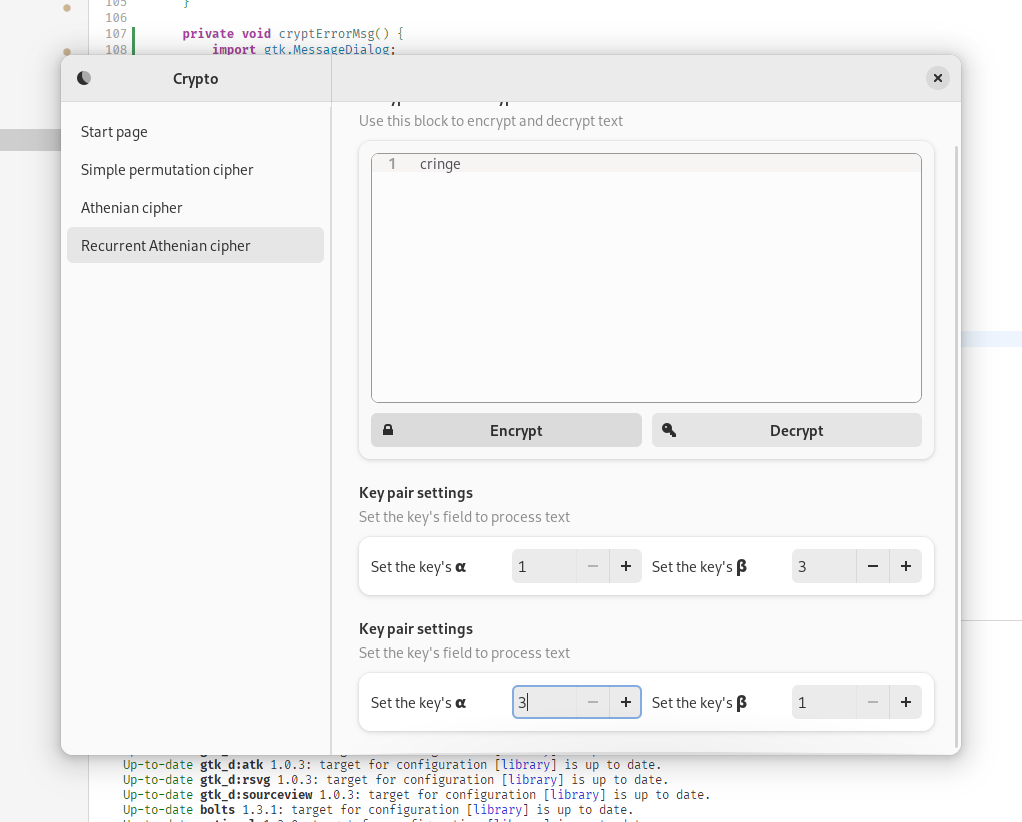
\includegraphics[width=0.8\textwidth]{01_0009}
    \label{img:0009}
  \end{figure}

  \begin{figure}[H]  
    \centering
    \caption{Зашифрование}
    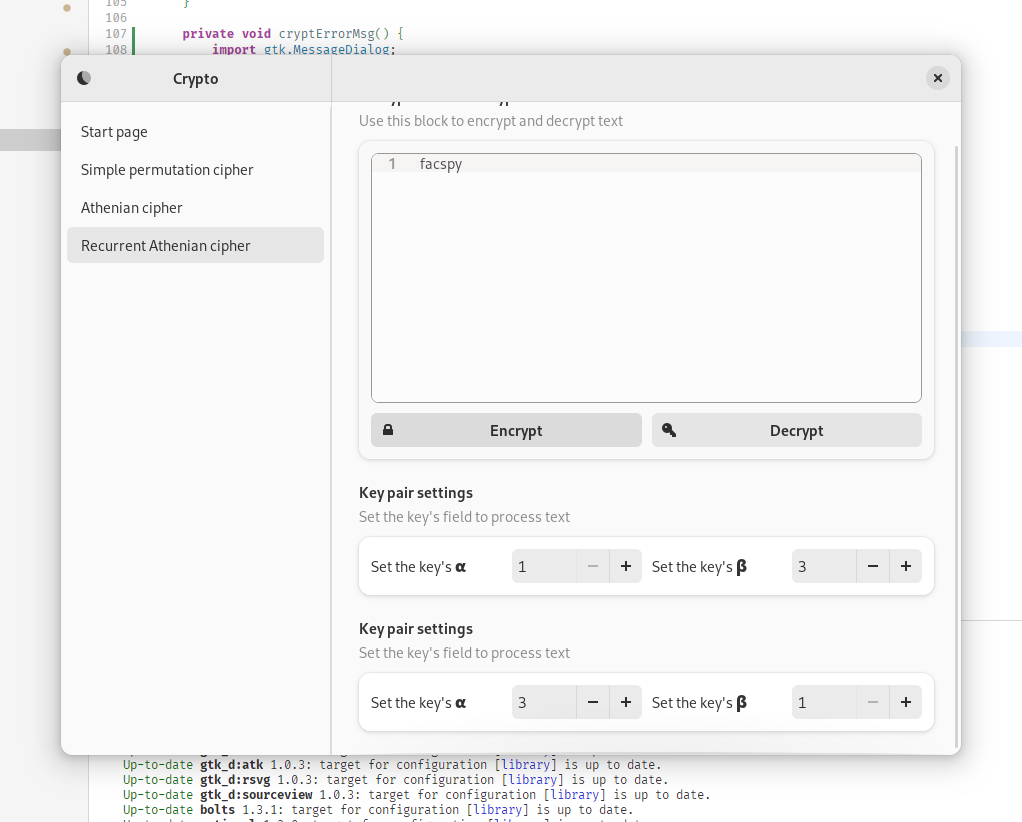
\includegraphics[width=0.8\textwidth]{01_0010}
    \label{img:0010}
  \end{figure}

  \begin{figure}[H]  
    \centering
    \caption{Расшифрование}
    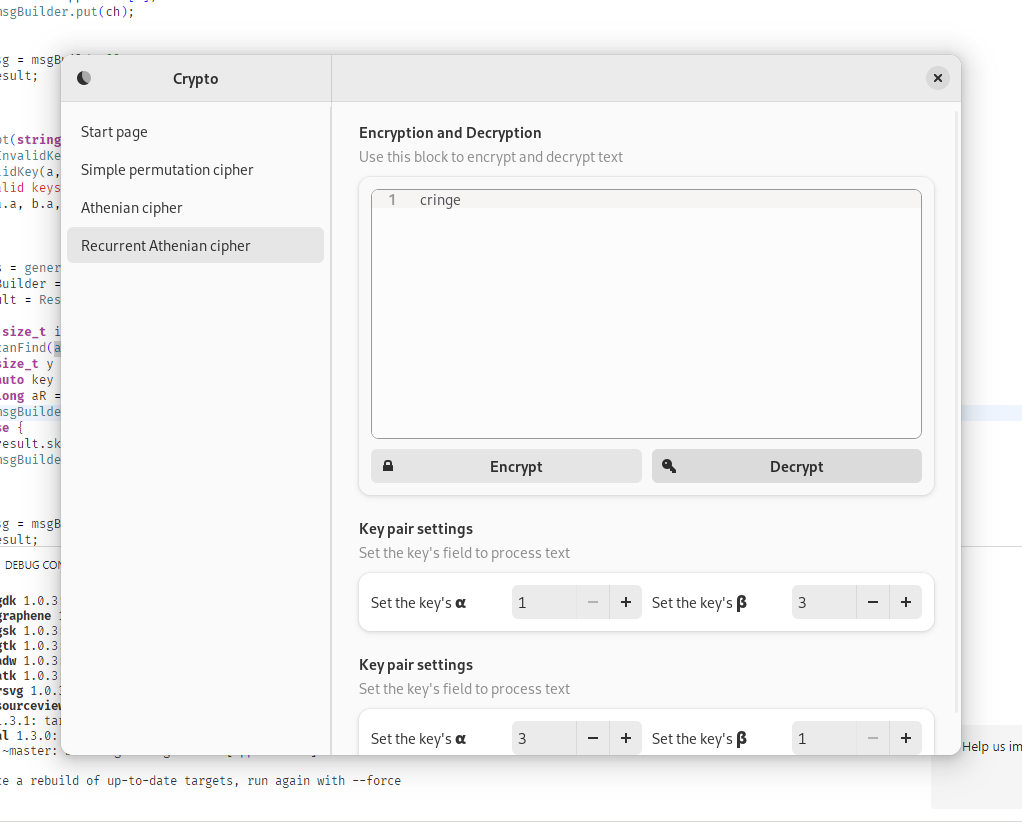
\includegraphics[width=0.8\textwidth]{01_0011}
    \label{img:0011}
  \end{figure}

  \newpage
  \section{Криптоанализ}

  \subsection{Метод грубой силы}

  Для шифра простой замены данный метод может быть весьма долгим и затратным, т.к. для алфавита 
  с длиной $n$ потребуется перебрать в худшем случае $n!$ возможных ключей. Поэтому данный шифр 
  не будет рассматриваться в данной секции.

  Для алфавита изместной длины достаточно просто реализовать полный перебор всех ключей для 
  Аффинного шифра, чуть сложнее для рекуррентного Аффинного шифра.

  Например, если исходный алфавит содержит 26 символов, то для подбора ключа Аффинного шифра 
  существуют 26 возможных значений $\beta$ и формально бесконечно возможное количество возможных 
  $\alpha$. Однако стоит учитывать тот факт, что НОД$(26, \alpha)$ должен быть равен единице,
  что позволяет быстро убрать из набора для перебора как минимум все числа, делящиеся на 2
  (для данного случая).
  
  \subsection{Частотный анализ}
  
  Частотному анализу подвержены шифр простой замены и Аффинный шифр, 
  это можно увидеть, благодаря гистограмме распределения частотности букв в тексте.

  Для этого возьмем какой-то не очень короткий текст и проведем над ним частотный анализ,
  зашифруем и проанализируем снова.

  \subsubsection{Шифр простой замены}

  \begin{figure}[H]  
    \centering
    \caption{Введем исходный текст}
    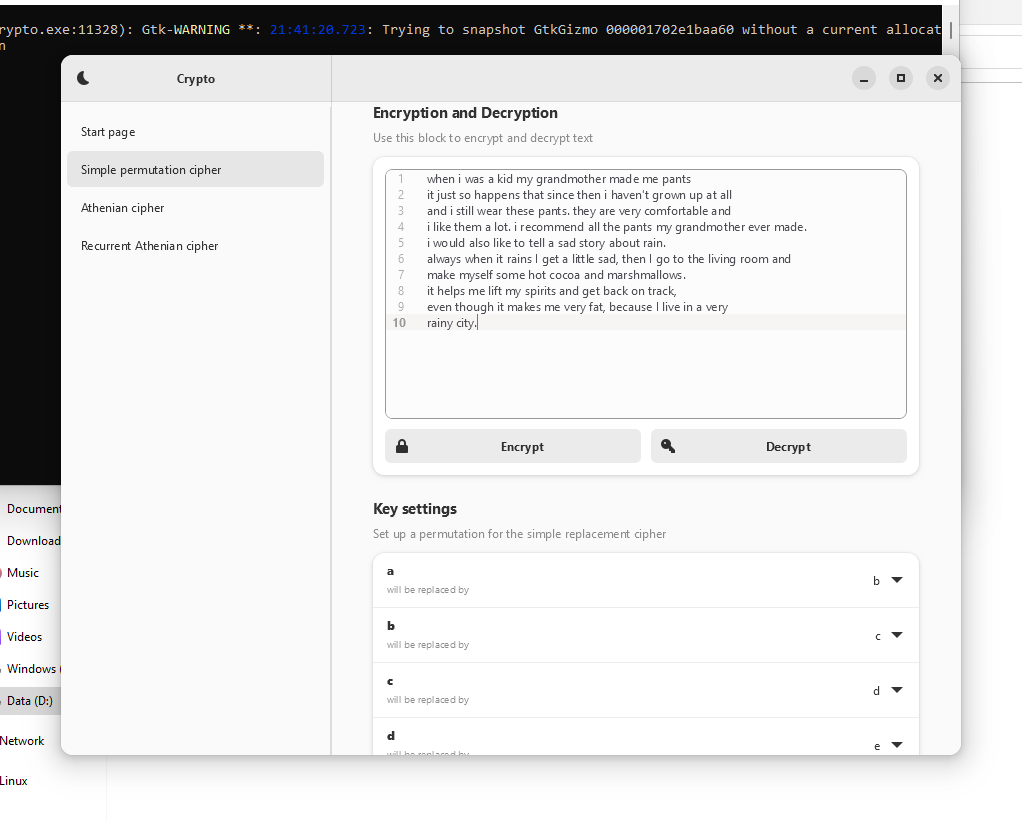
\includegraphics[width=0.75\textwidth]{01_0012}
    \label{img:0012}
  \end{figure}

  \begin{figure}[H]  
    \centering
    \caption{Проанализируем его}
    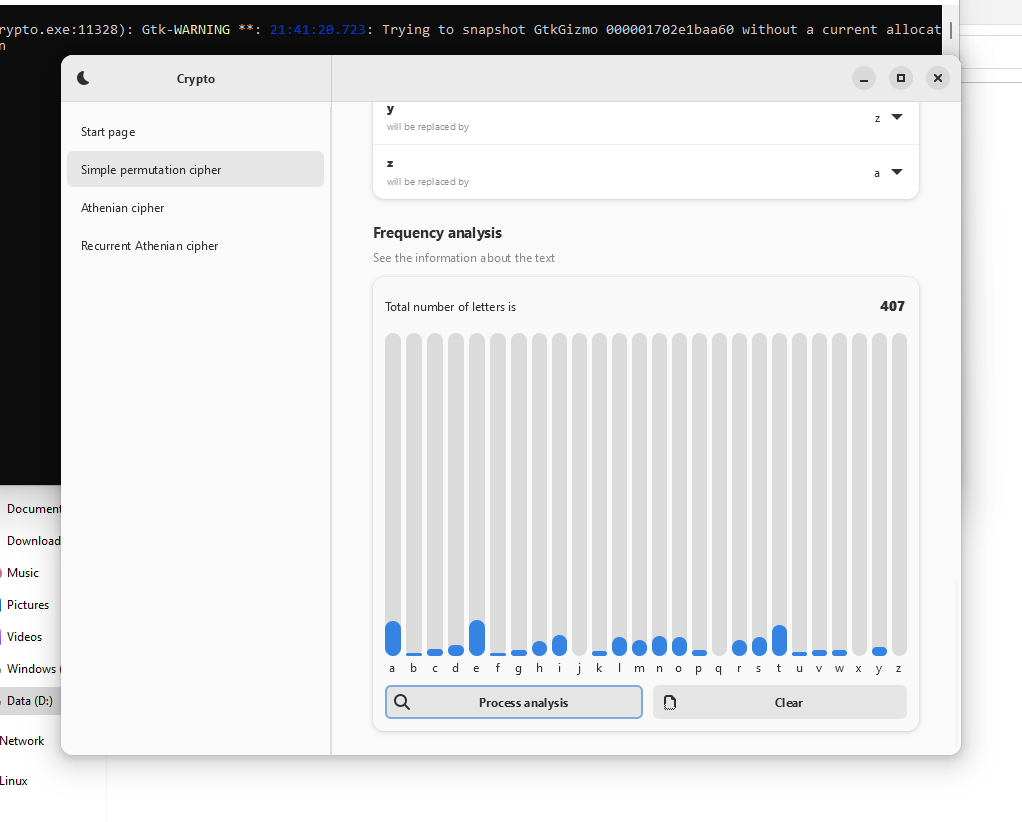
\includegraphics[width=0.8\textwidth]{01_0013}
    \label{img:0013}
  \end{figure}
  
  \begin{figure}[H]  
    \centering
    \caption{Зашифруем его}
    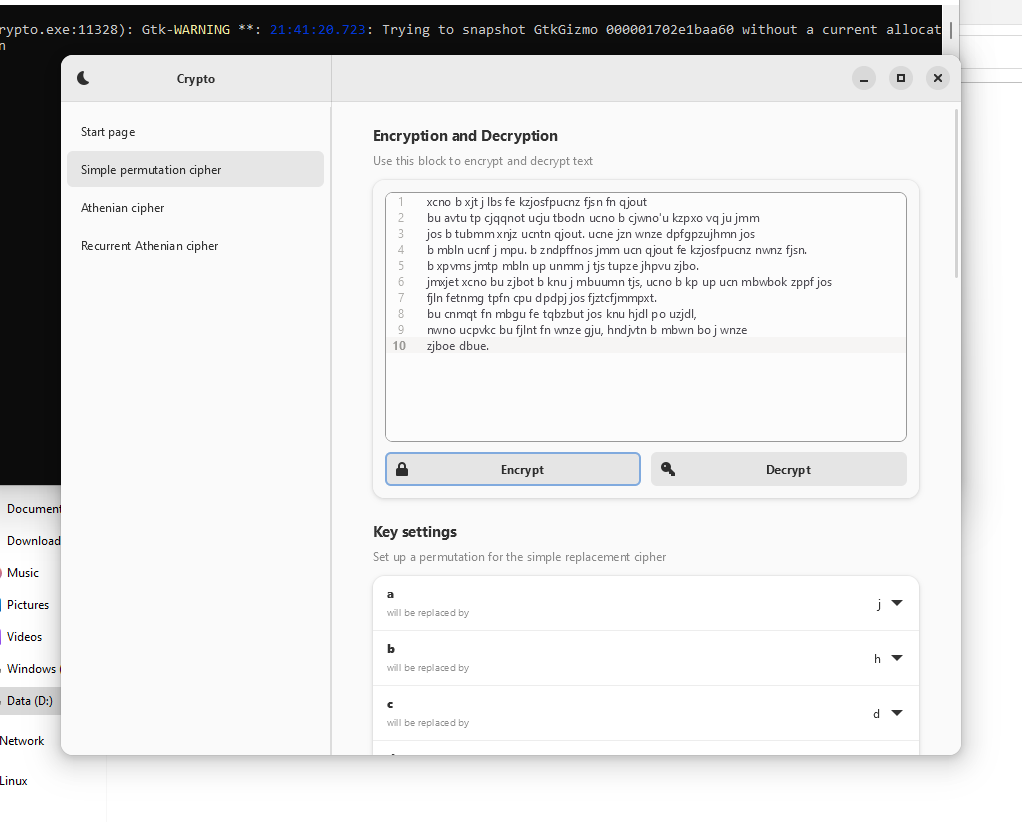
\includegraphics[width=0.8\textwidth]{01_0014}
    \label{img:0014}
  \end{figure}
  
  \begin{figure}[H]  
    \centering
    \caption{И снова проанализируем}
    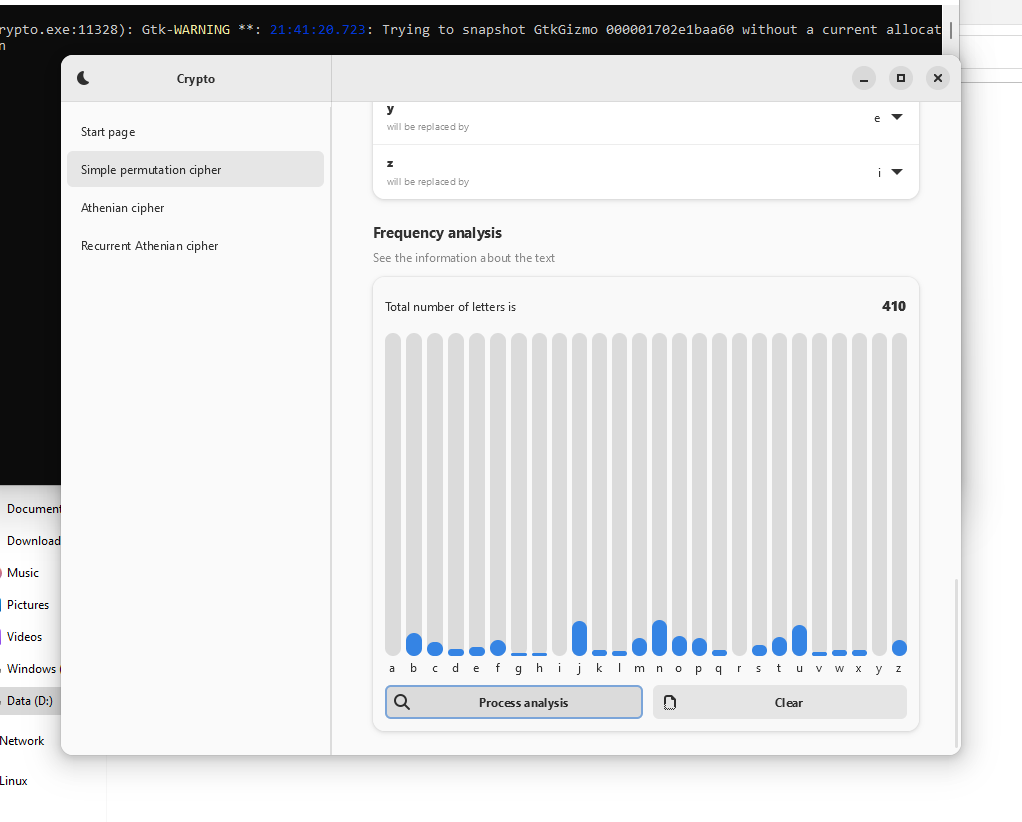
\includegraphics[width=0.8\textwidth]{01_0015}
    \label{img:0015}
  \end{figure}

  Как видно по гистограмме, численно значения не поменялись, поменялось лишь их 
  положение, что свидетельствует о том, что данный шифр действительно можно взломать
  с помощью частотного анализа.

  \subsubsection{Аффинный шифр}

  \begin{figure}[H]  
    \centering
    \caption{Рассмотрим исходный текст}
    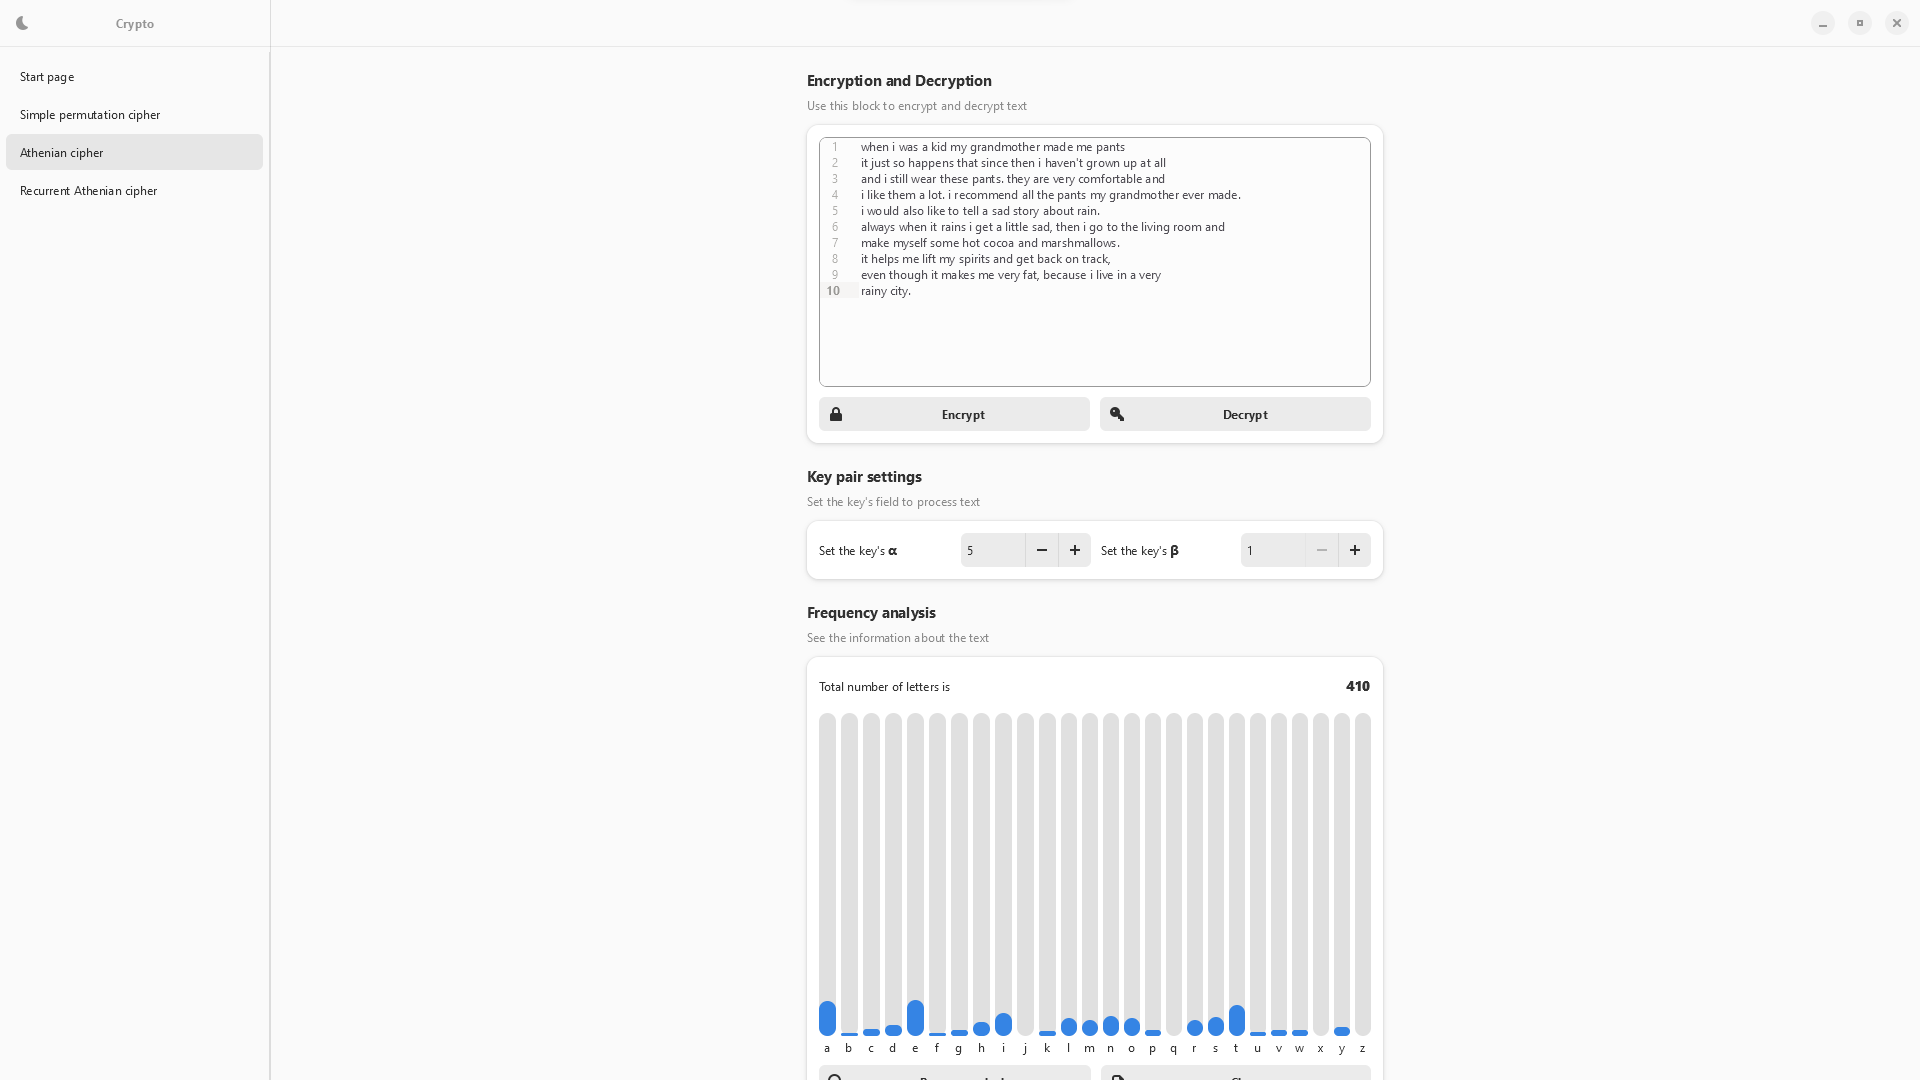
\includegraphics[width=0.8\textwidth]{01_0016}
    \label{img:0016}
  \end{figure}
  
  \begin{figure}[H]  
    \centering
    \caption{Рассмотрим зашифрованный текст}
    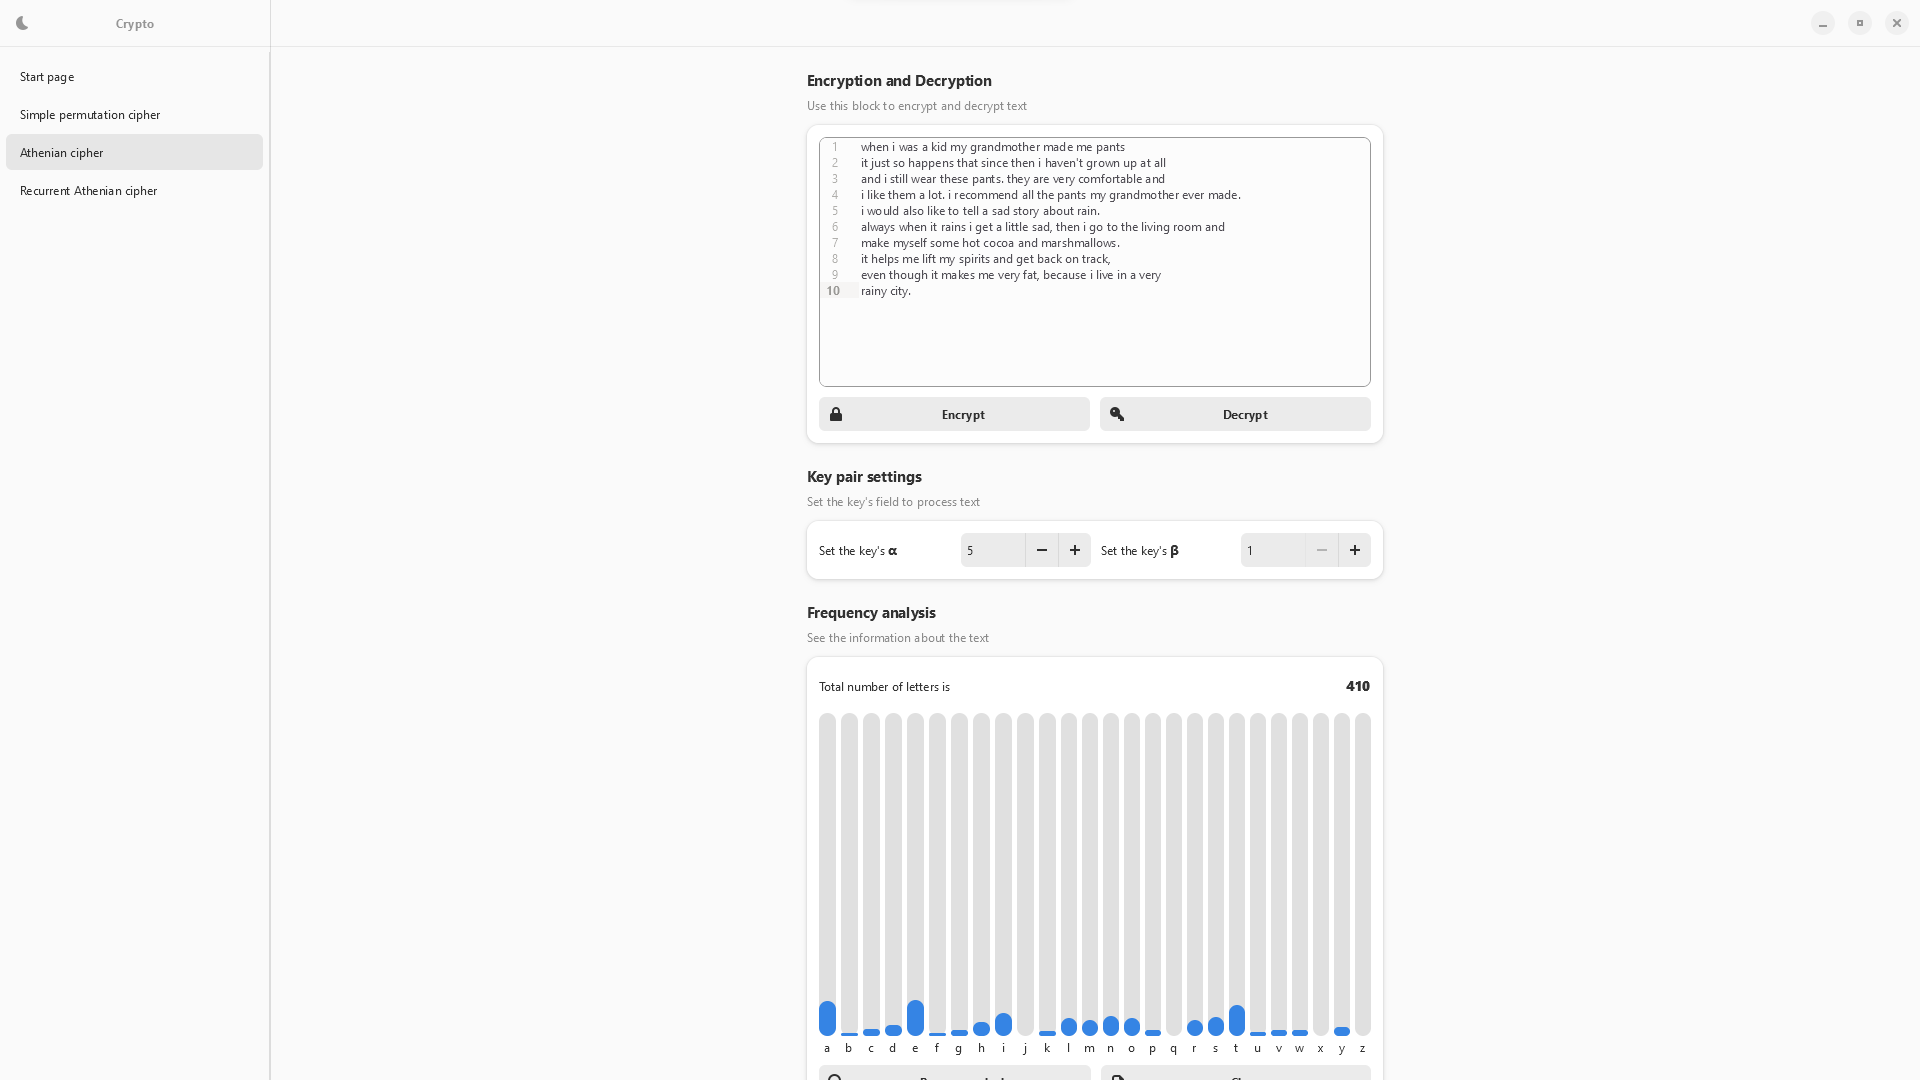
\includegraphics[width=0.8\textwidth]{01_0017}
    \label{img:0017}
  \end{figure}

  По гистограммам снова можно заметить, что шифр неустойчив к атакам, основанным на частотном анализе.
  
  \newpage
  \section{Вывод}

  В ходе данной практической работе были реализованны и протестированны следующие подстановочные 
  шифры - шифр простой замены, Аффинный шифр и рекуррентный Аффиный шифр.

  Шифр простой замены легок в реализации, устойчив к атаке методом грубой силы, однако легко 
  поддается криптоанализу. Его взлом может быть сильно упрощен, если злоумышленнику в руки 
  попадет часть исходного текста.

  Аффинный шифр легко поддается взлому любым из перечисленных методов: частотный анализ, метод грубой 
  силы, атака на основе открытого текста.

  Рекуррентный Аффинный шифр в отличие от всех остальных устойчив к частотному анализу,
  имеет более высокую защиту от атак на основе открытого текста, нежели обычный Аффинный шифр.
  Подвержен атаке методом грубой силы.
\end{document}
